\documentclass[chapterprefix=true, 11pt, a4paper, oneside, parskip=half, listof=totoc, bibliography=totoc, numbers=noendperiod]{scrbook}

\usepackage[bottom=32mm,left=25mm,right=25mm]{geometry}

\usepackage{scrhack}

\usepackage{blindtext}

\usepackage{caption}
\usepackage{subcaption}

\usepackage{imakeidx}

\usepackage{paralist}

\usepackage{epigraph}

\usepackage[toc, acronym]{glossaries}
\glsenablehyper

\usepackage[automark,headsepline]{scrlayer-scrpage}
\automark{chapter}
\ihead{\leftmark}
\chead{}
\ohead{\thepage}
\ifoot*{}
\cfoot[\thepage]{}
\cfoot*{}
\ofoot*{}
\pagestyle{scrheadings}


\usepackage[onehalfspacing]{setspace}

\usepackage[stretch=10]{microtype}

\usepackage[english]{babel}

\usepackage{lmodern}
\usepackage[utf8]{luainputenc}
\usepackage[T1]{fontenc}

\usepackage{epigraph}

\usepackage[printonlyused]{acronym}

\usepackage{float} 

\usepackage{tabularx}

\usepackage{longtable}

\usepackage{listings}

\usepackage[table,xcdraw]{xcolor}

\usepackage{tikz}

\usepackage{graphicx}

\usepackage{wrapfig}

%\usepackage{subfigure}

\usepackage[hidelinks,english]{hyperref}

\usepackage{csquotes}
\usepackage[style=alphabetic, backend=biber, bibencoding=utf8]{biblatex}
\addbibresource{references.bib}

\usepackage{amssymb}
\usepackage{amsmath}

\addtokomafont{disposition}{\rmfamily}

\usepackage{verbatimbox}
\newcommand\Includegraphics[2][]{\addvbuffer[5pt 0pt]{\includegraphics[#1]{#2}}}

\renewcommand{\lstlistlistingname}{Source Code Content}

\renewcommand*{\labelalphaothers}{}

\renewcommand{\lstlistingname}{Code snippet}

% Create a style for system calls 
\lstdefinestyle{syscalls}{
	language=C,
	columns=fullflexible,
	aboveskip=5pt,
	belowskip=10pt,
	basicstyle=\small\ttfamily,
	commentstyle=\color{teal},
	keywordstyle=\color{blue},
	stringstyle=\color{Ao},
	showspaces=false,
	showstringspaces=false,
	showtabs=false,
	xleftmargin=16pt,
	xrightmargin=0pt,
	framesep=5pt,
	framerule=0.5pt,
	frame=single,
	rulecolor=\color{black},
	tabsize=2,
	breaklines=true,
	breakatwhitespace=true,
	captionpos=b
}

\newglossarystyle{dottedlocations}{%
	\glossarystyle{list}%
	\renewcommand*{\glossaryentryfield}[5]{%
		\item[\glsentryitem{##1}\glstarget{##1}{##2}] \emph{##3}%
		\unskip\leaders\hbox to 2.9mm{\hss.}\hfill##5}%
	\renewcommand*{\glsgroupskip}{}%
}


% Titles Config - CHOOSE ONE SECTION for title format

%% Used for titleGraduation Bachelor
%% Based on https://ai-bachelor.htw-berlin.de/files/Stg/AI/richtlinie_ba-arbeit_ai_06_02_13.pdf
\makeatletter

\renewcommand*{\maketitle}{
	\begin{titlepage}
		\newgeometry{left=2.5cm,right=2.5cm,top=2.5cm,bottom=2.5cm}
		\begin{figure}[H]
			\centering
			
\includegraphics[width=0.5\textwidth]{images/htw/logo}
		\end{figure}
		\begin{center}
			\vfill
			{\Large System Calls for Containerising and Managing Processes in Linux\par}
			\vskip 0.5cm
			{\large \bfseries A Thesis\par}
			\vskip 0.5cm
			{\large Submitted in Partial Fulfillment of the Requirements for the
                    Degree of\vskip 0.5cm \bfseries Master of Science (M.Sc.) 
                    in Applied Computer Science}
			\vskip 0.5cm
			{\large at the}
			\vskip 0.5cm
			{\large Berlin University of Applied Sciences (HTW)}
			\vfill
			\begin{flushleft}
				\begin{tabular}[t]{rl}
					First Supervisor: & Prof. Dr. Sebastian Bauer\\
					Second Supervisor: & Dr. Michael Witt \\
					Author: & B.Sc. Atanas Denkov \\
					Matriculation Number: & s0559025 \\
					Submission Date: & 04.10.2022
				\end{tabular}
			\end{flushleft}
		\end{center}
		\restoregeometry
	\end{titlepage}
}
\makeatother


\makeindex[title=Index, options=-s indexstyle.ist, intoc]
\indexsetup{level=\chapter*,toclevel=chapter}

\makenoidxglossaries
\loadglsentries{glossary.tex}
\setacronymstyle{long-short}
\begin{document}

\pagenumbering{alph} % fix for same identifier warning, character is not show in title
\maketitle

\pagenumbering{roman}
\include{chapters/preface} \clearpage 
%\include{chapter/Abstract} \clearpage
%\include{chapter/Abstract_de} \clearpage

\tableofcontents \newpage

\pagenumbering{arabic}
\chapter{Introduction}
\section{Motivation}
Primitive support for multiprocessing in the form of basic context switching and dedicated input-output 
components was introduced in the late 1950s. Multiprocessing allowed for concurrent execution of 
multiple instructions at the cost of increased system complexity. Interleaved processes had a 
global unrestricted view of the system which inevitably led to unpredictable program behaviour. 
For example, programs had the ability to modify each other's memory and monopolise 
computer resources. Hence, to ensure correctness, every program had to carefully manage its interactions 
with hardware and all other processes in the system, which resulted in an unsustainable 
programming model.

The aforementioned issues were addressed by shifting the responsibility of resource management 
and process protection into a privileged control program that acted as an intermediary between 
hardware and user programs. This program is most commonly referred to as a kernel.
The centralisation of these tasks rendered the kernel an integral part of modern computing systems. 
The kernel is an essential part of a system's trusted computing base because it acts as a 
single point of failure for all user programs. This is a particularly important issue for 
infrastructure providers that sell high-availability execution environments where 
arbitrary, and therefore, untrusted applications from different tenants coexist.
If one application tampers with the kernel, then the whole system may potentially go down. 
Similarly, 
applications are able to tamper with each other, despite the protection mechanisms enforced 
by the kernel. To solve this problem, an additional level of indirection may be introduced between the tenant program
and all other programs on the system, including the kernel, that represents an unescapable 
execution environment, also called a virtual environment.

\section{Objectives}
The primary objective of this thesis is to conduct an experiment consisting of a set of 
synthetic workloads that measure response times and efficiency within a sandboxed environment.
The experiment executes the same workloads natively, within the standard noninterference boundary 
provided by the kernel to user space programs. The differences in response times and efficiency 
within and outside a container are used as an approximation of the overhead introduced 
by isolating a process from its environment. The experiment is reproducible and can be executed 
on any Linux system with a x86\_64 or arm64 compatible processing unit.

The second objective of this thesis is to design and implement a container runtime 
that will be used by the experiment as the primary sandboxing mechanism. The runtime's 
implementation, including the system calls that it relies on, will be thoroughly discussed and its security characteristics
will be qualitatively evaluated. 

\section{Content Structure}
Chapter \ref{ch:fundamentals} introduces the fundamental axioms, or trade-offs, in virtualisation technologies.
These will be referred to throughout the entire document. 
The same chapter also introduces the concept of resource namespaces - the primary abstraction 
provided by the kernel to sandbox processes.

Chapter \ref{ch:state-of-research} outlines the current state of research in operating-system 
virtualisation, highlights the relationships between noninterference, isolation and performance, and
discusses modern architectures that try to maximise all three.     

Chapter \ref{ch:concept} provides a detailed description of the requirements and the software architecture 
of the runtime, benchmark tool, and the workloads. The measurements to be sampled from the kernel are introduced.

Chapter \ref{ch:implementation} describes the implementation of the container runtime. Furthermore,
the security characteristics of the kernel's resource namespacing capabilities are discussed.

Chapter \ref{ch:Experiment} contains the performance evaluation experiment. First, the hardware 
platform under test is discussed. Second, a set of hypotheses are developed and proven and/or 
disproven with the help of the benchmark tool.  

Chapter \ref{ch:conclusion} contains conclusive remarks, a brief summary of the results of the thesis
and future work that can be done by other students in the field.  \clearpage
\chapter{Fundamentals}
\section{Virtualisation}
\subsection{Axioms}
\subsubsection{Isolation}
\textcite{10.1145/368481.368502} summarise the fundamental
requirements of a functional control program and emphasise the concept of noninterference between 
processes across space and time. Spatial and temporal noninterference can be seen as different 
qualitative measures of the control program's effectiveness to keep processes safe. Whereas the 
former deals with the mechanisms that protect references to memory, disk and I/O devices, the latter
deals with the allocation of execution time and the protection against the monopolisation thereof.

The STRETCH system \cite{10.1145/368481.368502}, albeit quite old, employs an architecture used by 
modern kernels to guarantee noninterference. The author describes an interruption system that can 
transfer execution to a different memory address whenever a condition of the machine or process 
changes, e.g an I/O device emits a signal or the process attempts divison by zero, respectively.
The address holds the start instruction of a privileged routine that can react to the changed 
condition. For example, the routine could serialise access to an I/O device, decode the bit stream 
and copy it into a memory block local to the process that issued the request. Serialising access 
ensures that concurrently executing processes cannot spatially interfere with the request. Scheduling
the next request to be processed so that all programs make equal or similar runtime progress guarantees 
temporal noninterference. It is important to note that, by definition, the kernel is considered 
trustworthy and is allowed to access and modify space assigned to user processes. Therefore, if it is
compromised or encounters an unrecoverable error condition, all user processes become untrustworthy 
or unavailable, respectively.

\textcite{10.1145/361011.361073} refer to the control program as a virtual machine monitor that 
ensures noninterference by providing every program with an environment that is \enquote{[...] effect
identical with that demonstrated if the program had been run on the original machine directly} 
\cite[2]{10.1145/361011.361073}. This definition implies that a running program, also called a 
\textit{virtual machine}, does not directly use the bare metal hardware resources available. Instead,
resources are emulated by the virtual machine monitor at the instruction-set level and presented as a
dedicated hardware system. \textcite{10.1145/361011.361073} define a requirement that the 
instruction-set architecture of a computer has to satisfy for it to be virtualisable. The instruction
set must be segregated into three groups of instructions - privileged, sensitive and innocuous. An 
instruction is privileged if it requires changing the mode of execution from user to supervisor mode 
by means of a trap. An instruction $i$ is control-sensitive if, when applied to the current processor
state $S_1$, results in a new state $i(S_{1}) = S_{2}$ such that the execution mode of $S_{2}$ does 
not equal that of $S_{1}$ or if $S_{2}$ has access to different resources than $S_1$ or both 
\cite{10.1145/361011.361073}. An instruction is behaviour-sensitive if its execution depends on the 
execution mode or its position in memory. An instruction is innocuous if it is not sensitive. Given 
these definitions, a computer is virtualisable \enquote{[...] if the set of sensitive instructions
for that computer is a subset of the set of privileged instructions} \cite[6]{10.1145/361011.361073}.
If this criterion is met, the virtual machine monitor can trap all sensitive instructions and emulate 
each via a homomorphism $i: C_{r} \rightarrow C_{v}$ that maps the state space of the processor without
the virtual machine monitor loaded $C_{r}$ to the state space with the virtual machine monitor loaded 
$C_{v}$. Innocuous instructions do not require protection, i.e a homomorphic mapping, and are directly
executed by the processor.


\subsubsection{Performance}
 \clearpage
\chapter{Appendix A}
\section{Hardware Virtualisation}
\label{ch:fundamentals/virtualisation/hardware-virtualisation}
\textcite{10.1145/361011.361073} refer to the control program as a \textit{virtual machine monitor} that 
ensures isolation and noninterference by providing every program with an environment that is \enquote{[...] effect
identical with that demonstrated if the program had been run on the original machine directly} 
\cite[2]{10.1145/361011.361073}. This definition implies that a running program does not directly use
the bare metal resources available. Instead, resources are emulated by the virtual machine monitor at
the hardware level and presented as a dedicated physical system. Such an environment is called 
a \textit{virtual machine}.

\begin{figure}[H]
    \centering
    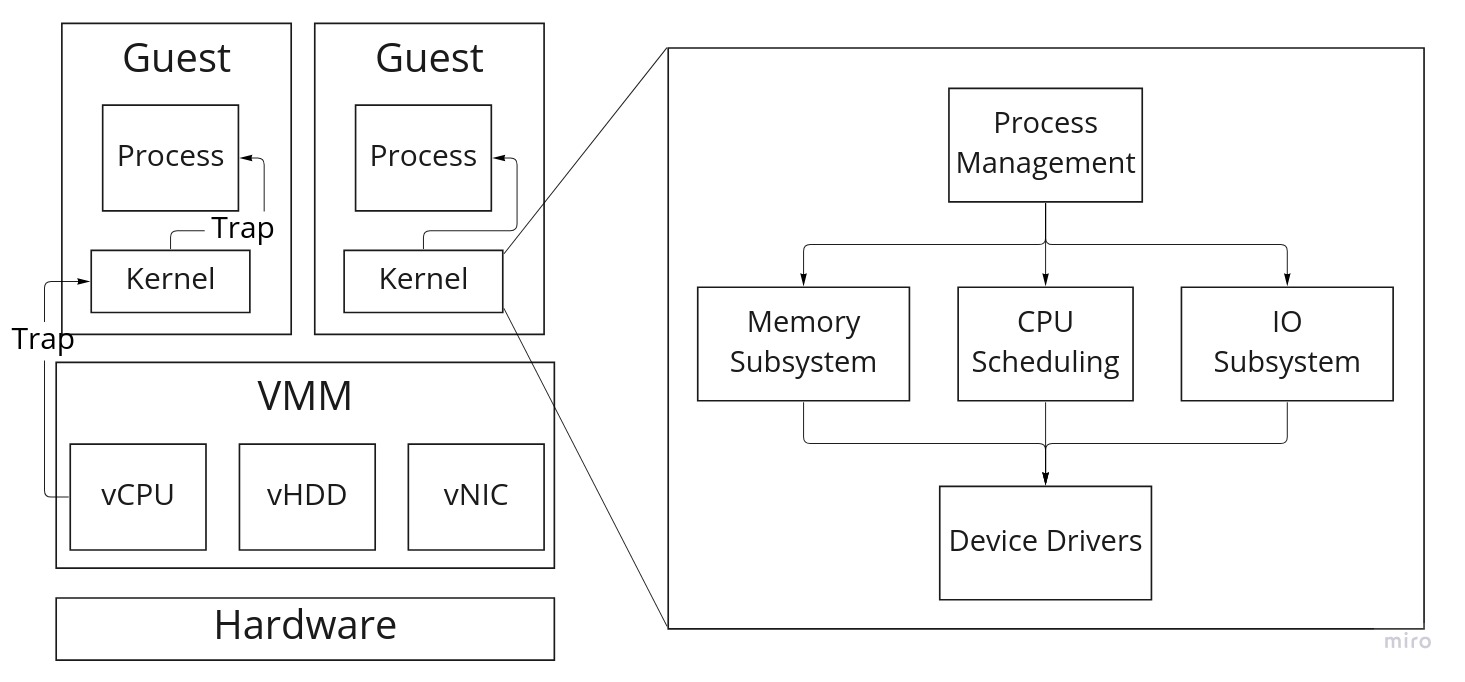
\includegraphics[width=0.70\textwidth]{images/fundamentals/full-virt-archh.jpg}
    \caption{Hardware virtualisation architecture. Each guest runs a complete operating system. 
             Privileged operations are trapped by the virtual machine monitor and emulated to provide hardware services.}
    \label{images:fundamentals/full-virt-archh.jpg}
\end{figure}

\textcite{10.1145/361011.361073} define a requirement that the instruction-set architecture of a computer
has to satisfy for it to be virtualisable. The instruction set must be segregated into three groups of
instructions - privileged, sensitive and innocuous. An instruction is privileged if it requires changing
the mode of execution from user to supervisor mode by means of a trap \cite{10.1145/361011.361073}. 
An instruction $i$ is control-sensitive if, when applied to the current processor state $S_1$, results
in a new state $i(S_{1}) = S_{2}$ such that the execution mode of $S_{2}$ does not equal that of $S_{1}$
or if $S_{2}$ has access to different resources than $S_1$ or both \cite{10.1145/361011.361073}. 
An instruction is behaviour-sensitive if its execution depends on the execution mode or its position
in memory \cite{10.1145/361011.361073}. An instruction is innocuous if it is not sensitive. 
Given these definitions, a computer is virtualisable \enquote{[...] if the set of sensitive instructions
for that computer is a subset of the set of privileged instructions} \cite[6]{10.1145/361011.361073}.
If this criterion is met, the virtual machine monitor can trap all sensitive instructions and emulate 
each via a homomorphism $i: C_{r} \rightarrow C_{v}$ that maps the state space of the processor without
the virtual machine monitor loaded $C_{r}$ to the state space with the virtual machine monitor loaded 
$C_{v}$ \cite{10.1145/361011.361073}. Innocuous instructions do not require protection, i.e a homomorphic
mapping, and are directly executed by the processor \cite{10.1145/361011.361073}.

Given the aforementioned homomorphism, a virtual machine can host a \textit{guest kernel} (Figure \ref{images:fundamentals/full-virt-archh.jpg}) that 
runs completely in user mode. 
Whenever the guest kernel attempts to execute a privileged instruction, 
the virtual machine monitor traps the attempt and emulates the instruction. 
Consequently, the guest kernel does not have to be a part of the trusted computing base. 
Even if it is compromised or encounters an unrecoverable error condition, other virtual machines 
remain unaffected. As a result, the isolation boundary between user programs running in different 
virtual machines is stronger compared to processes running on a shared kernel. 

In order to fully guarantee spatial noninterference between processes, the virtual machine monitor must 
be in full control of the host system's memory. There are two primary methods to do this - 
\textit{shadow paging} and \textit{extended page tables}. The former mechanism is considered first. 
The virtual machine monitor maintains a nested page table 
per guest, also called a \textit{shadow page table} \cite{10.5555/1204009}. 
In turn, the guest kernel maintains a page table per process. 
Whenever the guest kernel schedules a new process for execution, it modifies the \textit{page-table 
base register} to point to the page table for that process \cite{10.5555/1204009}. 
The virtual machine monitor intercepts this attempt and transparently updates the page table pointer to point to 
the guest's shadow page table corresponding to that process \cite{10.5555/1204009}. Note that 
the virtual machine monitor has to traverse the shadow page table for that guest in order to find the nested entry corresponding 
to the process. Afterwards, the memory management unit takes care of translating the virtual memory 
addresses of the guest and updating the \textit{translation lookaside buffer}.
Alternatively, the memory management unit may be \enquote{virtualisation-aware} in the sense that it knows 
there are two page tables it needs to traverse - the page table that maps guest virtual memory to guest 
\enquote{physical memory}, and the page table that maps guest physical memory to actual physical memory. 
The former is maintained by the guest kernel, whilst the latter is maintained by the virtual machine monitor.
The extended page table approach is up to 50\% faster than shadow paging \cite{2006PerformanceEO} because table
walks are done in hardware - by the memory management unit.
Nevertheless, maintaining page table data structures inside the virtual machine 
monitor and the guests leads to memory pressure, which is further amplified by the fact that 
guests, their applications and the virtual machine monitor all share the same physical memory \cite{10.5555/2490781}. 

The spatial noninterference property necessitates that the virtual machine monitor manage 
all input-output devices and their interactions with the guests. This is accomplished by the
already introduced trap-and-emulate pattern. When an application within a virtual machine 
issues a system call requesting some form of input-output, the request is processed by the 
I/O stack inside the guest. At the lowest level of the stack, the device driver issues a 
command to the device, typically by writing to memory specifically assigned to the device, or by
calling specific input-output instructions \cite{10.5555/2490781}. 
Either way, the virtual machine monitor intercepts this and traverses its own I/O stack, which 
remaps guest and real input-output addresses and forwards the request to a physical device \cite{10.1145/2063176.2063194}. 
After processing the request, the physical device triggers an interrupt that is caught by the virtual machine monitor and 
transformed into a virtual equivalent that is sent to the virtual machine that issued the request.
To reduce the overhead associated with interrupt processing, the virtual machine monitor can batch 
multiple events together and use a single interrupt to notify the guest kernel \cite{10.1145/2063176.2063194}.
Still, a request must traverse two input-output stacks. The same holds for the response.
In addition, hardware optimisations such as direct memory access are emulated in software, which 
further degrades performance. This, however, can be mitigated by integrating an input-output memory management 
unit that remaps all direct memory accesses of a device on the host to an address space in the guest.

The cost of hardware virtualisation becomes apparent when measuring same-host density
and boot times. \textcite{10.1145/3132747.3132763} consider memory consumption and on-disk image size
as the primary limiting factors. The authors measure the time it takes to create and boot
virtual machines using the Xen virtual machine monitor and show the negative effects that on-disk image size has 
by starting images with 
varying sizes by manually \enquote{[...] injecting binary objects into the uncompressed image file} \cite[3]{10.1145/3132747.3132763}. 
As the number of consolidated virtual instances increases and the image size grows, 
creation and boot times increase linearly.
Furthermore, the authors show that creating and starting a process directly on the host is, on average, 
two orders of magnitude faster. \textcite{10.1145/2151024.2151030} also evaluate Xen and state
that processing units spend 25\% of their total cycles in hypervisor mode instead of executing guest applications 
when running \enquote{[...] SPEC's first benchmark addressing performance evaluation of datacenter servers used in 
virtualised server consolidation} \cite[2]{10.1145/2151024.2151030}, which includes components 
such as a web, database and application server.

\section{Container configuration}

\begin{lstlisting}[style={syscalls}, label={code:oci-config.json}, caption={Open Containers Initiative Configuration File Example}]
{
    "process": {
        "args": [
        "nsbench-disk-workload"
        ],
        "cwd": "/"
    },
    "root": {
        "path": "./workloads/rootfs/disk",
        "readonly": false
    },
    "namespaces": [
        {
        "type": "user"
        },
        {
        "type": "net"
        },
        {
        "type": "ipc"
        },
        {
        "type": "mnt"
        },
        {
        "type": "uts"
        },
        {
        "type": "pid"
        }
    ],
    "uid_mappings": [
        {
        "container_id": 0,
        "host_id": 1000,
        "size": 1
        }
    ],
    "gid_mappings": [
        {
        "container_id": 0,
        "host_id": 1000,
        "size": 1
        }
    ],
    "hostname": "nsbench-disk-workload",
    "hooks": { 
        "on_runtime_create": [
            {
                "path": "/usr/bin/setup-network",
                "args": ["-a", "192.168.0.101"],
                "env": ["PATH=/usr/bin"],
                "timeout": 2
            }
        ],
        "on_container_created": [],
        "on_container_start": [],
        "on_container_started": [],
        "on_container_stopped": []
    }
}
\end{lstlisting}

\begin{lstlisting}[style=c-code-snippets, label={code:implementation/benchmark/network-hook-doer}, caption={Joining an arbitrary namespace, executing a function within it, and returing back to the original namespace}]
func DoInContainerNamespace(containerPid, namespace int, doer func() error) error {
    runtime.LockOSThread()
    defer runtime.UnlockOSThread()

    ns, ok := namespaces[namespace]
    if !ok {
        return ErrNamespaceUnsupported
    }

    oldNsPath := path.Join("/proc", "self", "ns", ns)
    oldNsFd, err := unix.Open(oldNsPath, unix.O_RDONLY|unix.O_CLOEXEC, 0)
    if err != nil {
        return err
    }
    defer unix.Close(oldNsFd)

    newNsPath := path.Join("/proc", strconv.Itoa(containerPid), "ns", ns)
    newNsFd, err := unix.Open(newNsPath, unix.O_RDONLY|unix.O_CLOEXEC, 0)
    if err != nil {
        return err
    }
    defer unix.Close(newNsFd)
    if err := unix.Setns(newNsFd, namespace); err != nil {
        return err
    }
    defer unix.Setns(oldNsFd, namespace)
    return doer()
}
\end{lstlisting}

\section{Netlink protocol}
\label{ch:appendix/netlink-protocol}

\clearpage
%\input{chapter/Analysis} \clearpage
%\input{chapter/Conception} \clearpage
%\input{chapter/Implementation} \clearpage
%\input{chapter/Test} \clearpage
%\input{chapter/Evaluation} \clearpage
%\input{chapter/Conclusion} \clearpage

\pagenumbering{Roman}
% List of Figures
\listoffigures \clearpage
% List of Tables
\listoftables \clearpage
% Source Code Content
\lstlistoflistings \clearpage

\printindex \clearpage

\printnoidxglossary[title=Glossar] \clearpage

\defbibfilter{scientific}{
	type=article or
	type=inbook or
	type=book or
	type=unpublished or
	type=inproceedings or
	type=incollection or
	type=manual or
	type=phdthesis
}

\printbibliography[heading=bibintoc, filter=scientific, title={References}]\clearpage
\printbibliography[heading=bibintoc, keyword={online}, title={Online References}]\clearpage
\printbibliography[heading=bibintoc, keyword={image}, title={Image References}]\clearpage

\end{document}
